\subsection*{Context of the internship}

As part of the \href{http://informatique.ens-lyon.fr/en/academic-programs/master/m1}{first year of Master} at the
\href{http://www.ens-lyon.fr/en/}{École Normale Supérieure de Lyon},
I was able to do a 12 weeks research internship in a laboratory.

My research for an internship in Quantum Algorithmic had brought me to
the \href{https://www.lu.lv/en/studies/faculties/faculty-of-computing/}{Faculty of Computing}
at the \href{https://www.lu.lv/}{University of Latvia}
and my supervisor \href{http://home.lu.lv/~ambainis/}{Andris Ambainis}. My research also
brought me to discuss with \href{https://kpfu.ru/Kamil.Hadiev?p_lang=2}{Kamil Khadiev}
from \href{https://eng.kpfu.ru/}{Kazan Federal University} who became my co-supervisor.
We discussed by email to find an interesting subject of research on which I
liked to work on. I thank them for their help, their supervision and the time they
gave to me during this 12 weeks.

During the internship, I have been integrated to the life of the
\href{https://quantum.lu.lv/}{Center for Quantum Computing Science}.
I thanks members of the team for the great discussions we had after
the seminar.

I also want to thank \href{https://perso.ens-lyon.fr/omar.fawzi/}{Omar Fawzi} for
having introduced me to quantum computing and its fascinating possibilities.

The team's research area is quantum algorithms and complexity theory. More precisely,
the team works on establishing new quantum algorithms with better complexity and proving
new bounds to the quantum complexity for many different types of problem belonging
from graph theory to cryptography passing by language recognition theory. My work on
the recognition of restricted Dyck words integrated itself great in the team work as it
has already been studied by the team for few years \cite{art:2DGrid} and further by
Kamil Khadiev \cite{DBLP:conf/uc/KhadievK21}.

My internship, named "Complexity of recognizing Dyck language with a
quantum computer", had for goal to reduce the gap between the lower and the upper bound for
the quantum query complexity of recognizing Dyck words of bounded height. The best
known lower and upper bounds are describe in \cite{art:2DGrid} by Andris Ambainis team.

In the end of the introduction, the field of research will be presented more precisely.
After that, technical preliminaries, which are useful to understand the
current and the new results, will be detailed. Finally, the last two sections present my
new results for the quantum query complexity of bounded height Dyck word and the different
tries to improve both upper and lower bounds.

\subsection{History of quantum computing}

The history of quantum computing has started in 1980 when Paul Benioff, an american physicist,
proposed a quantum mechanical model of Turing machines \cite{art:paulbenioff}.
His machine uses some properties of the matter that has been discovered by quantum physicists.
After that, some computer scientists suggested that the quantum model of Turing machines may be
more expressive that the classical model. Few years after, the first bricks of the quantum circuit
have been introduced by Richard Feynman \cite{art:feymann}. The first quantum computers have started
to arrived in the middle of 1990s. During the last 20 years, the funds given to the creation of
the first quantum computer have skyrocketed, as the number of start-ups and companies dedicated to it.
This emulation has made from the quantum computer field one of the most active field of research today.
On the algorithmic side, the first astonishing result is the algorithm designed by Peter Shor (1994)
\cite{art:shor}. The algorithm improves a lot the complexity of factorizing integers, enough to break our
cryptographic protocols when quantum computer will be powerful enough. Since 1994, the
quantum algorithm area has evolved almost independently from the quantum computers and
has developed many beautiful theories and interesting results. But first, how does a quantum
circuit works?

\subsection{The quantum circuit, and quantum query model and complexity}

In classical computer science, the piece of information is represented with
0 and 1. This two states can be easily obtained using electricity because 0
can be represented by 0V and 1 by 5V, it is easy to propagate electricity
through wires and to stock its level into capacitor. Moreover a little piece
of hardware, named transistor, has allowed to do some computations using logical
gates which once include in a complex machine create our so-called "computers".

For quantum computers, the story isn't so different. First, the 0 and 1 are
now represented using particles like electrons or photons. For example,
an electron with a spin of $+\frac{1}{2}$ (noted \ket{1}, pronounced ket 1) represents a 1 and
an other one with a spin of $-\frac{1}{2}$ (noted \ket{0}, pronounced ket 0) represents a 0.
But the use of particles is motivated by their properties and mainly by
a quantum property called superposition. A quantum state is not only \ket{0}
or \ket{1}, but can be both in the same time, i.e.
$\lambda_0 \ket{0} + \lambda_1 \ket{1}$ for every $\lambda_{0, 1} \in \mathbb{C}$
such that $\vert\lambda_0\vert^2+\vert\lambda_1\vert ^2=1$. A quantum bit,
called qubit, correspond to a quantum state that is a superposition of two
value. As before, the computations are done by gates, here
quantum gates, which transform the quantum state of a qubit into another
quantum state.
At the end, to get the result of a computation, it is mandatory to measure the
state of the quantum system, which breaks the quantum superposition. A quantum
state of $n$ qubits can be represented with a vector in a $2^n$
dimensional space whose norm is equal to 1, and a quantum gate by a linear
unitary transformation on a $2^n$ dimensional space. A transformation is said
unitary if it preserved the lengths.

\paragraph*{A quantum circuit} is a precise configuration of quantum gates
on a finite number of qubits. The following \autoref{fig:quantum_circuit_examle}
represents the quantum circuit that computes a uniform randomize on $\{0, 1\}^n$.

\begin{figure}[h!]
    \begin{minipage}{.30\textwidth}
        \centering
        $
            \Qcircuit @C=.8em @R=1em {
            \mbox{$n$ \textrm{entries}} &     &                              &     & \mbox{$n$\ \textrm{outputs}}    \\
            \lstick{\ket{0}} & \qw & \multigate{2}{H^{\otimes n}} & \qw & \meter & \cw\\
            \vdots & & \ghost{H^{\otimes n}} & \qw & \vdots &\\
            \lstick{\ket{0}}& \qw & \ghost{H^{\otimes n}} & \qw & \meter & \cw\\
            }$
    \end{minipage}
    \hfill
    \begin{minipage}{.65\textwidth}
        \textbf{Legend:}

        $ \bullet \
            \Qcircuit @C=1em @R=1em {
            & \qw & & \cw \\
            }$ are respectively a quantum wire and a classical wire.

        $\bullet \ \Qcircuit @C=.4em @R=.4em {
            & \gate{H^{\otimes n}} \\
            }$ is the Hadamard's gates on each input qubit.

        $\bullet \ \Qcircuit @C=.4em @R=.4em {
            & \meter \\
            }$ is the measure of 1 qubit in the algorithm.
    \end{minipage}
    \caption{A quantum circuit computing the uniform random on $\{0, 1\}^n$. }
    \label{fig:quantum_circuit_examle}
\end{figure}

\paragraph*{The quantum query circuit} is a quantum circuit used to
compute function on an entry $x=x_1 \ldots x_N$ that belongs to an entry space.
The black box model \cite{black_box_andris} of a quantum query circuit is composed of
an input state $\ket{\psi_ {start}}$ and a sequence
$U_0, Q, U_1, \ldots, Q, U_T$ of linear unitary transformations such that $\ket{\psi_{start}}$ and all $U_i$
do not depend on entry $x$ unlike the $Q_i$ which depend on $x$. The quantum state
$\ket{\psi_ {start}}$ belongs to a $d$-dimensional space generated
by $\ket{1}, \ket{2},\ldots, \ket{d}$.  To define $Q$, the basis vectors first need to
be renamed from $\ket{1},\ldots, \ket{d}$ to $\ket{i, j}$ with
$i \in \llbracket 0, N\rrbracket$ and $j \in \llbracket1, d_i \rrbracket$ for some
$d_i$ such that  $d_1 + d_2 + \ldots + d_N = d$. Next, $Q$ is define such that

\[Q(\ket{i, j}) := \left\{
    \begin{array}{ll}
        \ket{0, j}  & \textrm{if\ } i = 0                           \\
        \ket{i, j}  & \textrm{if\ } i > 0 \ \textrm{and\ } x_i = 0  \\
        -\ket{i, j} & \textrm{if\ } i > 0 \ \textrm{and\ } x_i = 1.
    \end{array}
    \right.  \]

The gates $Q$ are doing the queries to input $x$ by flipping some of the vectors.
Finally, to get the output of the quantum query algorithm it is necessary to
measure the output. A quantum query algorithm can the summarized with the following
quantum circuit.

\begin{figure}[h!]
    \centering
    $
        \Qcircuit @C=.8em @R=1em {
        \lstick{\vdots} & \qw & \multigate{2}{U_0}  & \multigate{2}{Q} & \multigate{2}{U_1} & \qw &  & &  \multigate{2}{Q} & \multigate{2}{U_T}&\multigate{2}{\metersymbol{.2}} & \cw\\
        &\lstick{\ket{\psi_{start}}} qw & \ghost{U_0} & \ghost{Q} & \ghost{U_1} & \qw & \cdots & & \ghost{Q} & \ghost{U_T} & \ghost{\metersymbol{.2}}& \cw\\
        \lstick{\vdots}& \qw & \ghost{U_0} & \ghost{Q}  & \ghost{U_1} & \qw & & &\ghost{Q} &\ghost{U_T}&\ghost{\metersymbol{.2}}& \cw \\
        }$
    \caption{Structure of a quantum query algorithm.}
    \label{fig:quantum_query_algorithm_structure}
\end{figure}

\paragraph*{The quantum query complexity} of an algorithm corresponds to the number of calls to the $Q$ gate. Often, this number of calls
is depending on the size of the entry. The quantum query complexity of a problem corresponds to the highest possible bound for which it is
certain there is no quantum query algorithm with a lower quantum query complexity solving the problem.

\subsection{Dyck Languages of height $k$}

First, the Dyck language corresponds to the set of correct and balanced words of parenthesis.
Often, computer scientist used another more graphical and convenient definition where
parenthesis words are replaced with discrete paths onto a 2D space. Indeed, every path starts
at coordinate $(0, 0)$ and is composed of 2 types of steps: The first one is an increasing step
that is represented  by adding to the end of the current path the vector $\overrightarrow{ (1,1)}$.
The second one is an decreasing step, it works similarly but the add vector is $\overrightarrow{ (1,-1)}$.
Moreover, to be a Dyck path, the path should start with an increasing step, it should never cross
the abscise axis and it should finish on it. A Dyck word of length 12 is presented in \autoref{fig:dyck_word}.
The Dyck language is a context free language as it can easily be recognized using a context
free grammar. The work done by Andris Ambainis' team \cite{art:2DGrid} focus on a restriction
on Dyck language with bounded height $k$. More precisely, a Dyck word is of height at most $k$ if, in every
of its prefix, the difference between the number of opening and closing parenthesis does not
exceeds $k$. In the path representation, a path is said to be of height at most $k$ if the path
never cross the line $y = k$. \autoref{fig:dyck_word} illustrates two different Dyck words with
only one of height at most 3. The restricted Dyck language with bounded height $k$ is noted \Dyck{k}
and is interesting because it belong to the already well studied class of star
free languages (Detail in \autoref{ssec:starfree}).

\begin{figure}[h!]
    \centering
    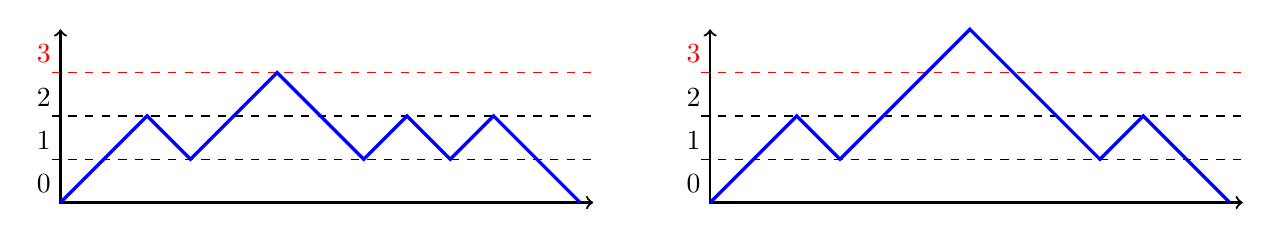
\begin{tikzpicture}[scale=.55]
        \draw[<->, thick] (0, 4) -- (0, 0)  -- (12.3, 0);
        \draw[dashed] (-.2, 1) -- (12.3, 1);
        \draw[dashed] (-.2, 2) -- (12.3, 2);
        \draw[dashed, red] (-.2, 3) -- (12.3, 3);
        \draw[blue, very thick] (0, 0) -- (2, 2) -- (3, 1) -- (5, 3) -- (7, 1) -- (8, 2) -- (9, 1) -- (10, 2) -- (12, 0);
        \draw (0, 0) node[above left] {0};
        \draw (0, 1) node[above left] {1};
        \draw (0, 2) node[above left] {2};
        \draw[red] (0, 3) node[above left] {3};

        \draw[<->, thick] (15+0, 4) -- (15+0, 0)  -- (15+12.3, 0);
        \draw[dashed] (15+-.2, 1) -- (15+12.3, 1);
        \draw[dashed] (15+-.2, 2) -- (15+12.3, 2);
        \draw[dashed, red] (15+-.2, 3) -- (15+12.3, 3);
        \draw[blue, very thick] (15+0, 0) -- (15+2, 2) -- (15+3, 1) -- (15+6, 4) -- (15+9, 1) -- (15+10, 2) -- (15+12, 0);
        \draw (15+0, 0) node[above left] {0};
        \draw (15+0, 1) node[above left] {1};
        \draw (15+0, 2) node[above left] {2};
        \draw[red] (15+0, 3) node[above left] {3};
    \end{tikzpicture}
    \caption{\textbf{On the left}, a valid Dyck word of height at most 3. \textbf{On the right}, an invalid Dyck word of height at most 3.}
    \label{fig:dyck_word}
\end{figure}

\subsection{State of the art}
This state of the art is not too precise as the understanding of the
bibliography took almost the first half the internship and is
more detail in \autoref{sec:preli}. First, few years ago Aaronson,
Grier and Schaeffer \cite[2019]{trichotomy_not_andris} worked on quantum query complexity
of recognizing regular languages as they can model a lot of tasks. They
concluded that there are 3 different cases depending of the language:
\begin{itemize}
    \item $O(1)$ if it is sufficient to read constant number of letters at the beginning and the end.
    \item $\tilde{\Theta}(\sqrt{n})$ if a Grover's search\footnote{
              The Grover search is a quantum query algorithm that allows to
              search for a marked element in a set of $n$ elements, where $p$ of them are marked,
              with a quantum query complexity of $O(\sqrt{\frac{n}{p}})$.
          } is the best way to recognize the language. The tilde refers to the existence of a
          constant $c_{te}$ such that the quantum query complexity is
          equal to $\Theta \left(\sqrt{n}(\log_2(n))^{c_{te}}\right)$.
    \item $\Theta(n)$ if recognizing the language is the same as counting modulo some value that can
          be computed with $O(n)$.
\end{itemize}
Further more, it is proved that being in the second classes is equivalent to
being a star-free language. Andris Ambainis' team decided to work on \Dyck{k} as this
language is a beautiful example of star-free languages. In \cite[2020]{art:2DGrid},
the team focused on finding the value of $c_{te}$, the power of the logarithm, in order
to find the exact quantum query complexity.
They first proved by reduction that the quantum query complexity of \Dyck{k}
called $Q\left(\Dyck{k}\right)$ is in $\Omega\left(c^k\sqrt{n}\right)$ where $c$ is
a constant greater than 1. They also gave an algorithm for \Dyck{k} with a quantum
query complexity of $O\left(\sqrt{n}(\log(n))^{0.5k}\right)$. Since then, no better
lower bound or algorithm have been found.

\subsection{Goals of the internship}
The problem on the quantum query complexity of \Dyck{k} is still open, my internship
has for goal to reduce the gap between the lower bound and the best known algorithm.
My researches have been organized on two main axes:
\begin{itemize}
    \item \textbf{Increasing the lower bound.} To do this, it is necessary to understand the bibliography
          on the adversary method in order to try to find a new adversary with better property. An other
          way is to use already existing lower bounds and translates them to \Dyck{k} with reductions.
    \item \textbf{Lowering the upper bound.} It is sufficient to find new algorithms
          with a better quantum query complexity than the previous ones. As for lower bounds,
          reduction method can also provides interesting new upper bounds.
\end{itemize}
Finally, the overall goal would be to made the two bounds match in order to get the exact quantum
query complexity of \Dyck{k}.

\subsection{Results}

The main results of my internship are presented in \autoref{main_section}. The first
one is a small revision of the original quantum query algorithm that recognize
\Dyck{k} \cite{art:2DGrid} and the second one is a new quantum query algorithm
for \Dyck{2} and its modifications to improve more the already revised original
algorithm.